\documentclass[unicode, 14pt, aspectratio=169]{beamer}
\usepackage{bussproofs}
\usepackage{listings}
\usetheme{titechen}
\addbibresource{main.bib}
 \date{\today}
\title{The Origins of Type Theory}
\author{\texttt{ryotaro612}}
\newcommand\blfootnote[1]{%
  \begingroup
  \renewcommand\thefootnote{}\footnote{#1}%
  \addtocounter{footnote}{-1}%
  \endgroup
}

\begin{document}
\begin{frame}[noframenumbering, plain]
\titlepage
\end{frame}
\section{Introduction}
\begin{frame}
  \frametitle{Objective}
  {\large Introduction to fields related to the theory of types}
  \par
  \vspace{16pt}
  Fields related to the references of this slides
  \begin{itemize}
  \item Logic
  \item Set theory
  \item Semiotics
  \item Structuralism
  \item Philosophy of language
  \end{itemize}
\end{frame}
\section{Non-euclidean geometry}
\begin{frame}
  \frametitle{Geometry in ancient Greece}
  {\large The approach to develop Geometry in ancient Greece was deductive reasoning.}
\begin{columns}
  \begin{column}{0.25\textwidth}
    \begin{center}
      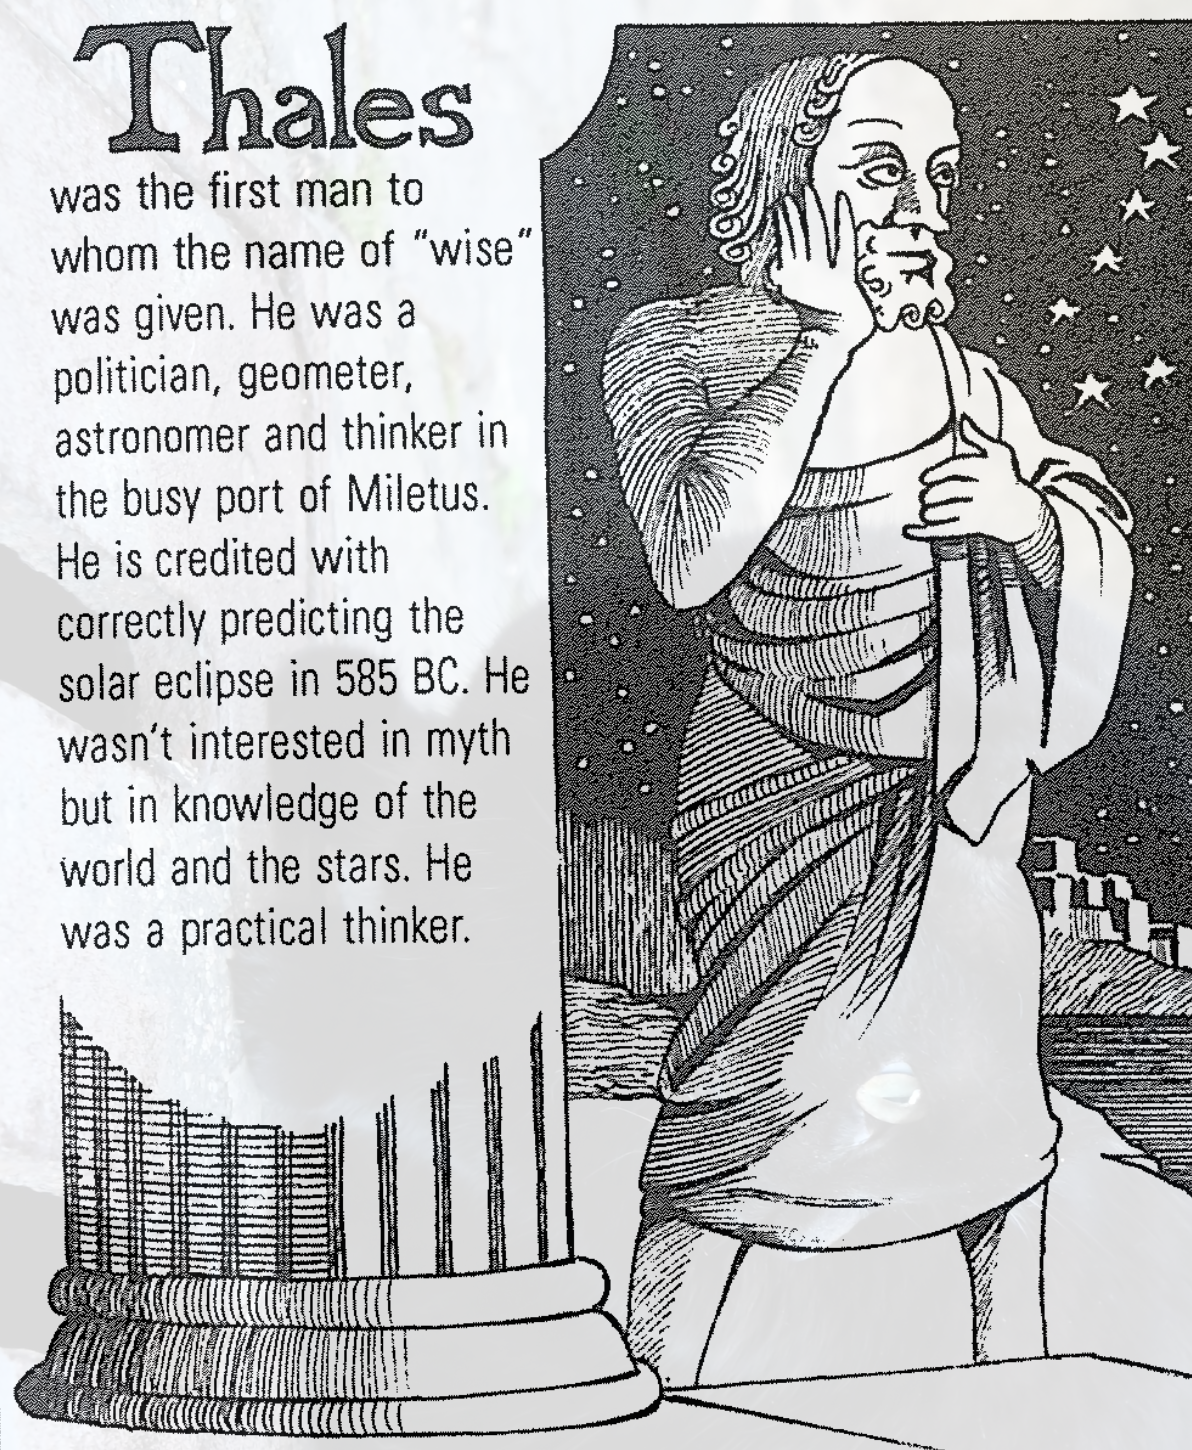
\includegraphics[width=0.7\textwidth]{images/thales.png}
    \end{center}
  \end{column}
  \begin{column}{0.25\textwidth}
    \begin{center}
      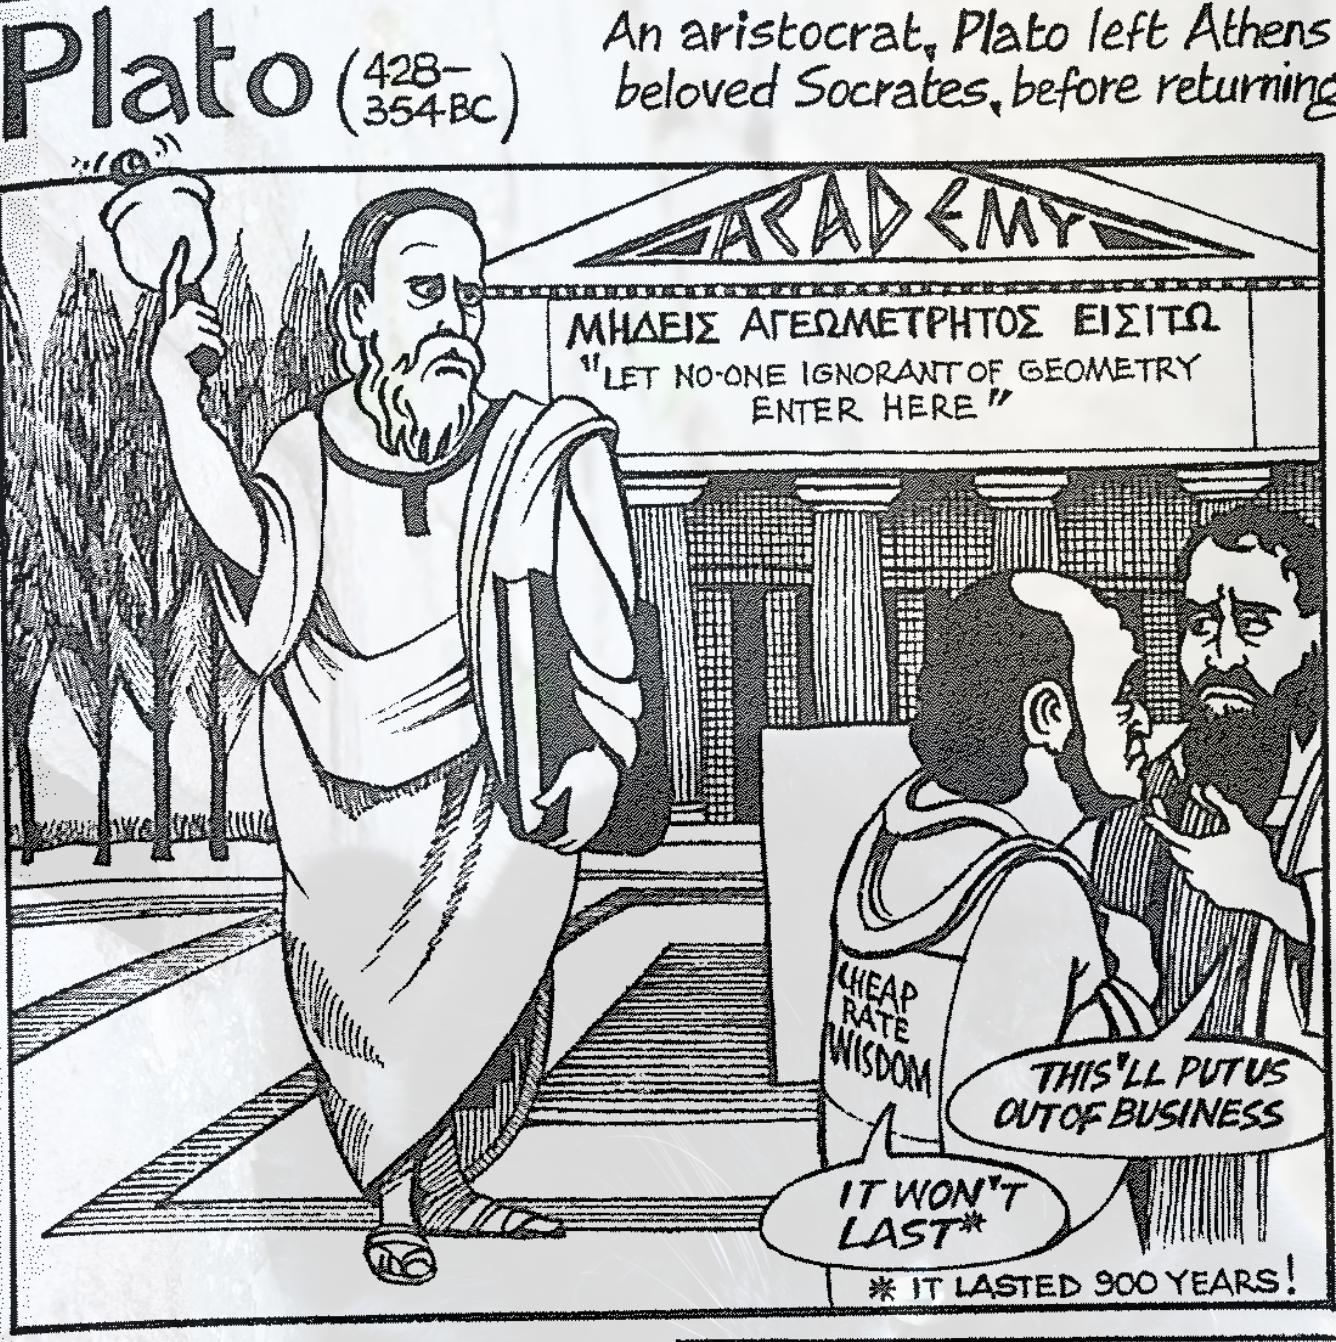
\includegraphics[width=0.7\textwidth]{images/plato.png}
    \end{center}
  \end{column}
  \begin{column}{0.25\textwidth}
    \begin{center}
      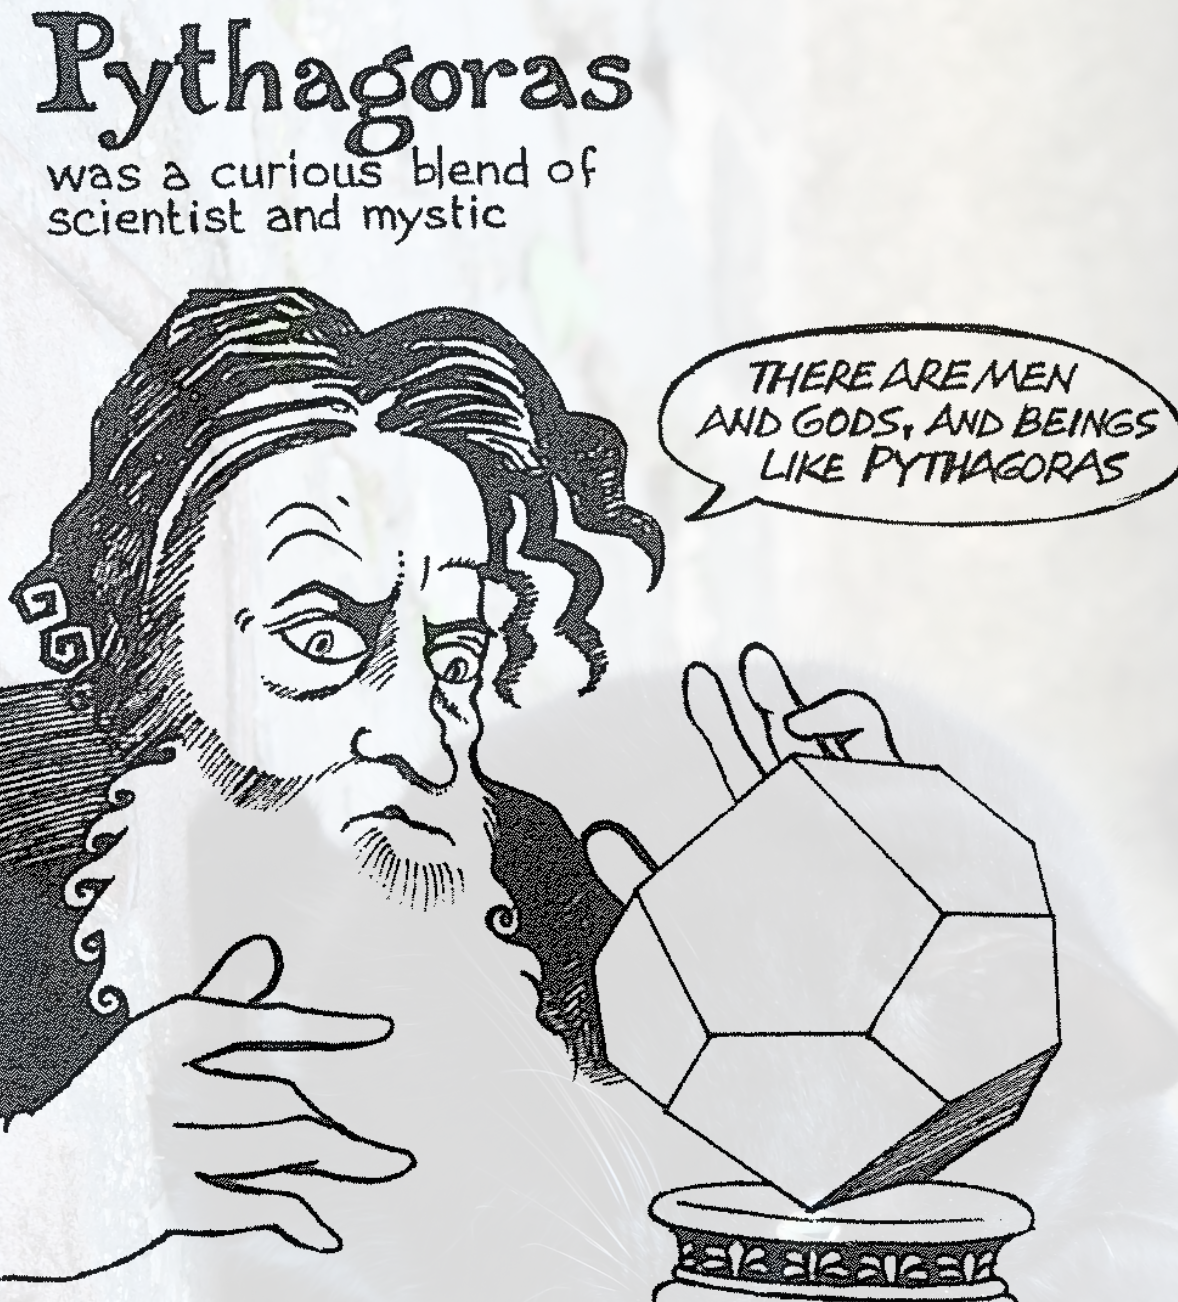
\includegraphics[width=0.7\textwidth]{images/pythagoras.png}
    \end{center}
  \end{column}
  \begin{column}{0.25\textwidth}
    \begin{center}
      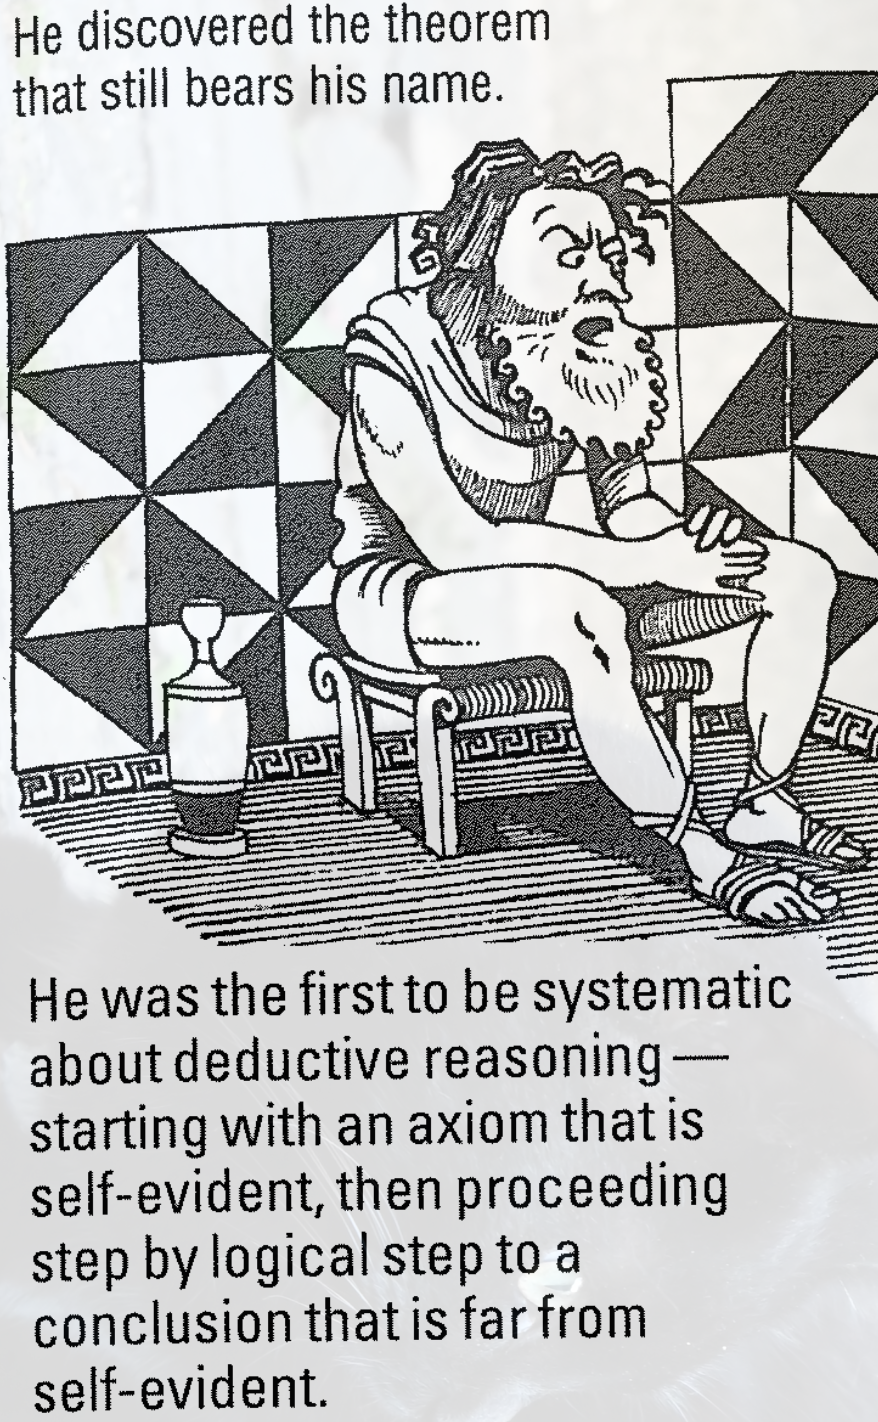
\includegraphics[width=0.7\textwidth]{images/pythagoras2.png}
    \end{center}
  \end{column}  
\end{columns}
\blfootnote{Images adapted from Philosophy for beginners\supercite{philosophy-for-begginers}}
\end{frame}
\begin{frame}
  \frametitle{Euclid's Elements}
  {\large Euclid's Elements is a collection of axioms, postulates, propositions, and proofs.}
  \par
  \vspace{16pt}
  \begin{description}[leftmargin=0cm]
  \item[Definition 1] A point is that of which there is no part.
  \item[Definition 2] A line is a length without breadth.
  \item[Definition 3] A surface is that which has length and breadth only.
  \item[Axiom 5] The whole is greater than the part.
  \end{description}
\end{frame}
\begin{frame}
  \frametitle{Euclid's postulates}
  {\large The fifth postulate never seemed self-evident.}
  \par
  {\footnotesize
  \begin{enumerate}
  \item Let it have been postulated to draw a straight-line from any point to any point.
  \item To produce a finite straight line continuously in a straight line.
  \item To draw a circle with any center and radius.
  \item All right-angles are equal to one another.
  \item If a straight-line falling across two straight-lines makes internal angles on the same side less than two right-angles, then the two (other) straight-lines, being produced to infinity meet on that side (of the original straight-line) that the (sum of the internal angles) is less than two right-angles (and do not meet on the other side).
  \end{enumerate}
  }
\end{frame}
\begin{frame}
  \frametitle{The fifth postulate is known as the parallel postulate.}
  {\large Given a straight line and a point not on that line, there is exactly one straight line parallel to the original line that passes through the given point.}
  \blfootnote{Figure adapted from 「数学の世界史」\supercite{suugaku-no-sekaishi}}
  \begin{figure}
    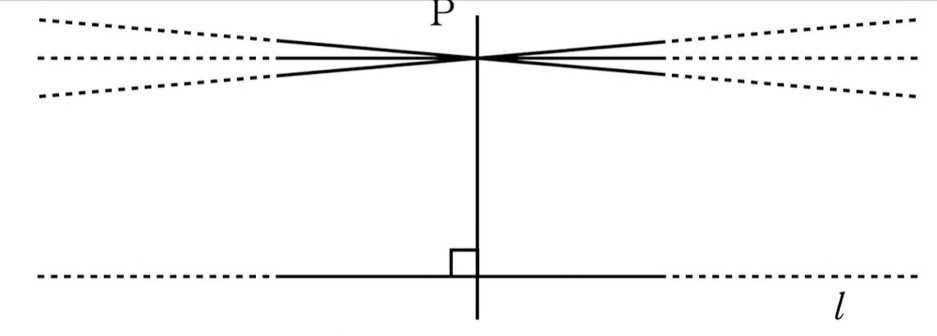
\includegraphics[width=0.6\textwidth]{images/axiom5.png}
    \caption{A parallel line and a point $p$ not on that line}
  \end{figure}
\end{frame}
\begin{frame}
  \frametitle{Investigations of the parallel postulate}
  \begin{itemize}
  \item Many attempts were made to derive the parallel postulate using the rest of the other postulates.
    \begin{itemize}
    \item Investigations were made by Alhazen (965-1039) and Khayyam (1048–1131).
    \item The Saccheri-Legendre Theorem states that if the parallel postulate is not assumed, then the sum of the angles of a triangle is less than or equal to 180 degrees.
    \end{itemize}
  \item The negation of the parallel postulate leads to no contradiction with the other postulates.
    \begin{itemize}
      \item Lobachevsky (1792-1856), along with János Bolyai (1802-1860), independently proposed a system where many parallels exist, leading to no contradictions within the geometry itself.
    \end{itemize}
  \end{itemize}
\end{frame}
\begin{frame}
  \frametitle{Non-Euclidean geometries}
  {\large For instance, in spherical geometry, great circles on a sphere intersect at exactly two points.}
  \blfootnote{Figure adapted from "はじめての構造主義"\supercite{structure}}
  \begin{figure}
    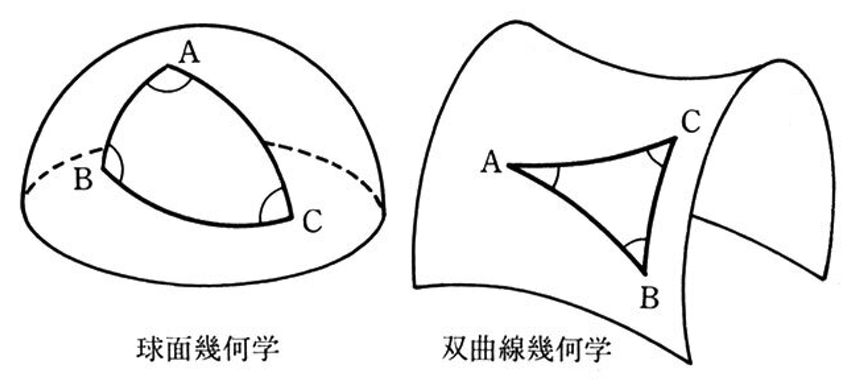
\includegraphics[width=0.4\textwidth]{images/non-euclid.png}
    \caption{Spherical space and hyperbolic space}
  \end{figure}
  In spherical geometry, a great circle corresponds to a straight line in Euclidean geometry.
\end{frame}
\section{Naive set theory}
\begin{frame}
  \frametitle{The development of set theory}
  {\large The discovery of non-Euclidean geometry inspired a rethinking of mathematical foundations}
  \begin{itemize}
  \item The discovery led mathematicians to have the idea that mathematics could be constructed on various axiom systems.
  \item Georg Cantor developed set theory as a foundational framework for mathematics, providing a unified approach to handle different mathematical concepts. 
  \end{itemize}
\end{frame}
\begin{frame}
  \frametitle{A unified approach}
  {\large A sketch of how to constrcut mathematical concepts using only the emtpy set.}
  \par
  \begin{enumerate}
  \item Begin with the empty set, denoted by $\emptyset$, $\{x|x\neq x\}$.
  \item Define the successor function $ S(n) = n \cup \{n\} $, which essentially adds one to a number by creating a new set.    
  \item Define $\emptyset$ as 0: $ 0 = \emptyset$.
  \item 1 is defined as $S(0) = \{ \emptyset \}$.
  \item 2 as $S(1) = \{ \emptyset, \{ \emptyset \} \}$.
  \item Continue this process to generate all natural numbers.    
  \end{enumerate}
\end{frame}
\section{Mathematical logic}
\begin{frame}
  \frametitle{Logicism}
  {\large Frege developed predicate logic and employed it and set theory to provide a logical basis for arithmetic.}
  \begin{columns}
    \begin{column}{0.8\textwidth}
      \begin{itemize}
        \item In "The Foundations of Arithmetic," Frege aimed to show that the truths of arithmetic are derived from logical axioms.
      \item In "On Sense and Reference," Frege distinguished between sense and reference.
        \begin{itemize}
        \item The terms "Morning Star" and "Evening Star" have different senses but share the same reference.
        % \item This distinction helps explain how different expressions can convey different cognitive values while referring to the same object.
        \end{itemize}
      \end{itemize}
    \end{column}    
    \begin{column}{0.2\textwidth}
      \begin{figure}
        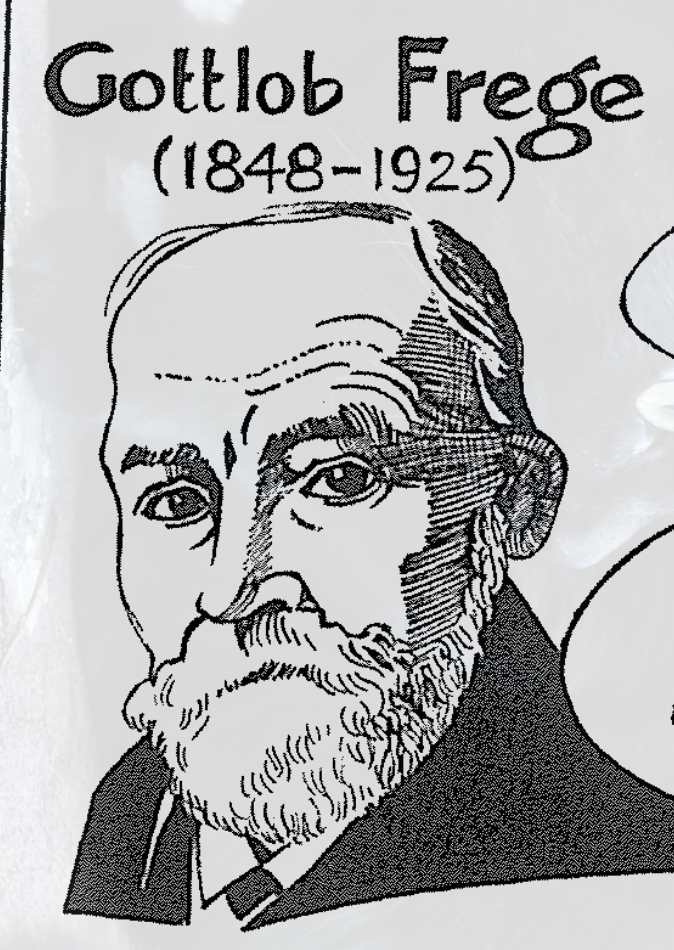
\includegraphics[width=1\textwidth]{images/frege.png}
      \end{figure}       
    \end{column} 
  \end{columns}
  \blfootnote{Figure adapted from Philosophy for beginners\supercite{philosophy-for-begginers}}
\end{frame}

\begin{frame}
  \frametitle{Leibniz's pioneering work in symbolic manipulation}
  {\large The approach to calculate inference by manipulating symbols was already explored in the 17th century.}  
  \begin{columns}
    \begin{column}{0.55\textwidth}
      {\setlength{\leftmargini}{0.05\paperwidth}
       \setlength{\leftmarginii}{16pt}
      \begin{itemize}
        \item Calculus derivatives
        \item The binary number system
        \item characteristica universalis
          \begin{itemize}
          \item a universal system of signs to eliminate the ambiguity of natural nlanguage by developing an alphabet of human thoughts
          \end{itemize}
        \end{itemize}
      }
    \end{column}    
    \begin{column}{0.4\textwidth}
      \begin{figure}
        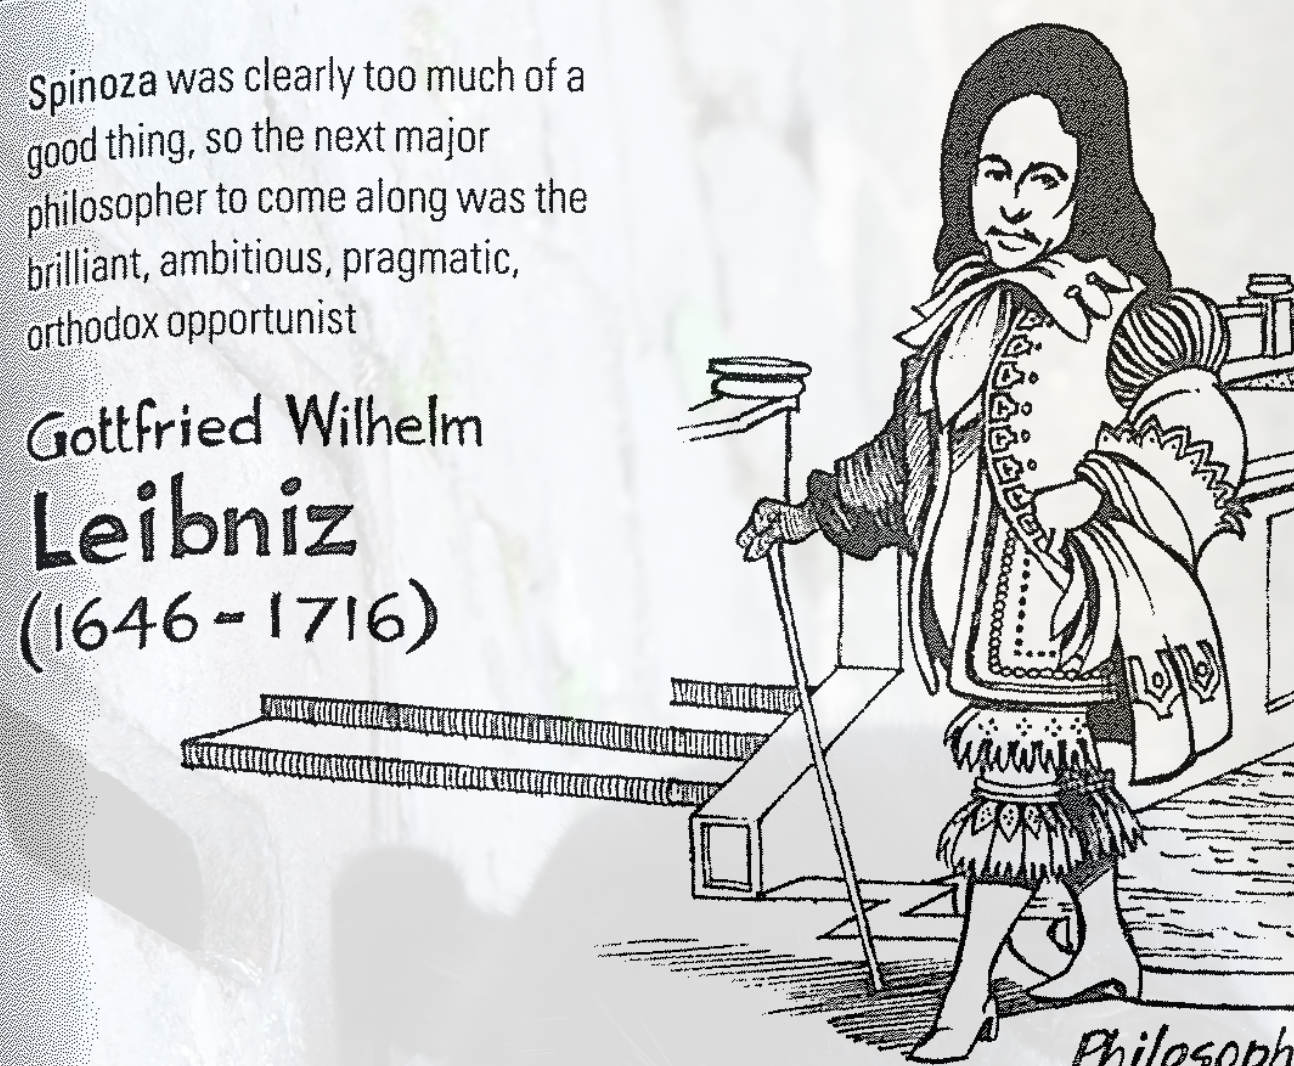
\includegraphics[width=0.65\linewidth]{images/leibniz.png}
        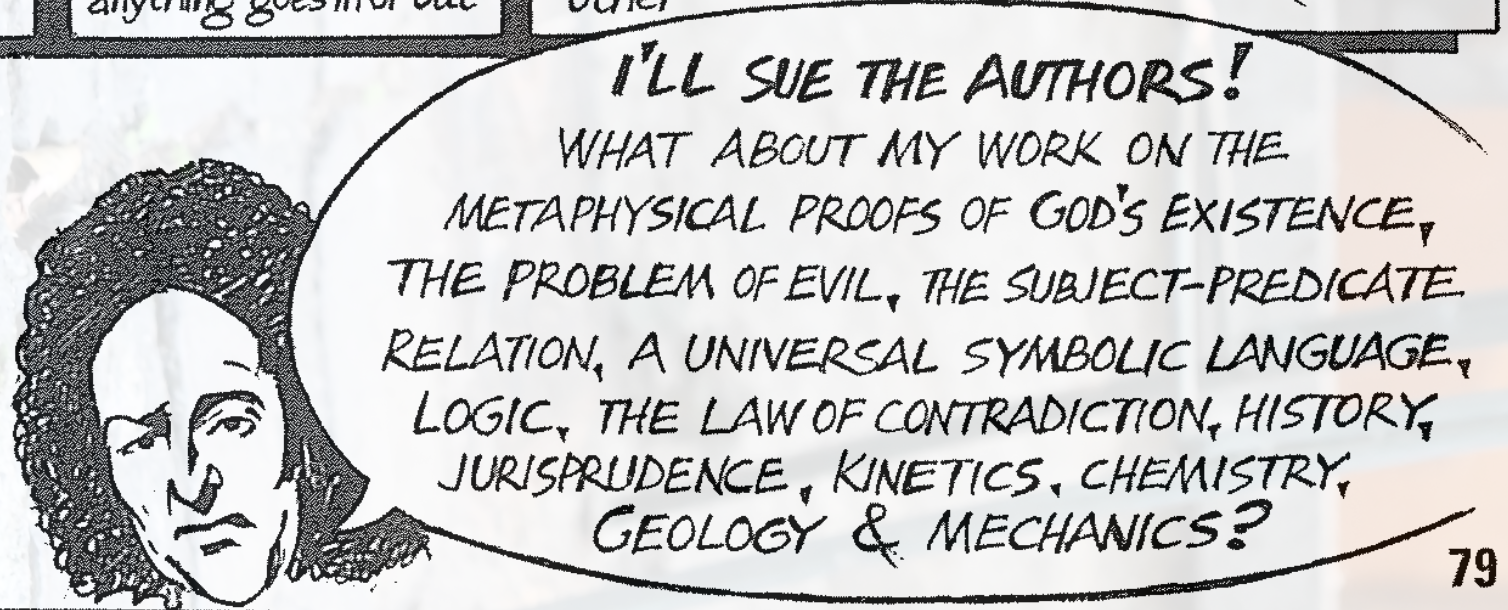
\includegraphics[width=0.65\linewidth]{images/universal.png}
      \end{figure}
    \end{column} 
  \end{columns}
  \blfootnote{Figures adapted from Philosophy for beginners\supercite{philosophy-for-begginers}}  
\end{frame}
\begin{frame}
  \frametitle{Boole Turned Logic into Algebra}
  {\large Boole employed symbols to represent classes of individuals in propositions.}
  \begin{columns}
    \begin{column}{0.7\textwidth}
      \begin{center}
        "The Laws of Thought"\supercite{bool}
        \begin{quotation}
          Let us then agree to represent the class of individuals to which a particular name or description is applicable, by a single letter, as x. If the name is “men,” for instance, let x represent “all men,”
        \end{quotation}
      \end{center}
    \end{column}    
    \begin{column}{0.2\textwidth}
      \begin{figure}
        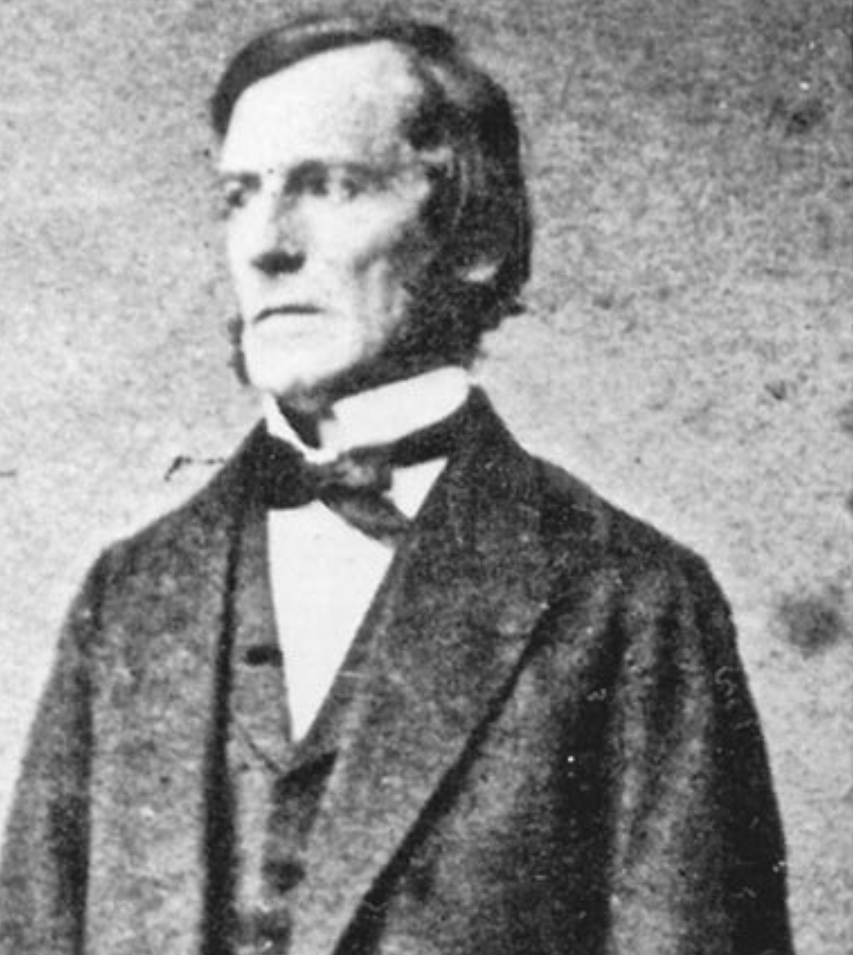
\includegraphics[width=1\textwidth]{images/bool.png}
      \end{figure}       
    \end{column} 
  \end{columns}
  \blfootnote{Figure adapted from "The Universal Computer: The Road from Leibniz to Turing"}
\end{frame}
\begin{frame}
  \frametitle{Propositional Logic}
  {\large Propositional logic involves using statements and deducing their truth based on logical connectives.}
  \par
  \vspace{16pt}
  {\small
  \AxiomC{$\varphi, \psi$}
  \RightLabel{(\wedge I)}
  \UnaryInfC{$\varphi\wedge\psi$}
  \DisplayProof
  \AxiomC{$\varphi\wedge\psi$}
  \RightLabel{(\vee E)}
  \UnaryInfC{$\varphi$}
  \DisplayProof
  \AxiomC{$\varphi\wedge\psi$}
  \RightLabel{(\vee E)}
  \UnaryInfC{$\psi$}
  \DisplayProof
  \AxiomC{$[\varphi]$}
  \noLine
  \UnaryInfC{$\vdots$}
  \noLine
  \UnaryInfC{$\psi$}
  \RightLabel{(\rightarrow I)}  
  \UnaryInfC{$\varphi\rightarrow\psi$}
  \DisplayProof
  \AxiomC{$\varphi$}
  \AxiomC{$\varphi\rightarrow\psi$}
  \RightLabel{(\rightarrow E)}  
  \BinaryInfC{$\psi$}
  \DisplayProof
  \AxiomC{$\bot$}
  \RightLabel{($\bot$)}
  \UnaryInfC{$\varphi$}
  \DisplayProof
  \AxiomC{$[\neg\varphi]$}
  \noLine
  \UnaryInfC{$\vdots$}
  \noLine
  \UnaryInfC{$\bot$}
  \RightLabel{(RAA)}
  \UnaryInfC{$\varphi$}
  \DisplayProof
  }
  \par
  a proposition is a declarative statement that is either true or false but not both.
\end{frame}
\begin{frame}
  \frametitle{Conceptual Notation}
  {\large Frege formalized statements with predicates.}
  \begin{itemize}
  \item Statements like “$\varphi$ is ~” are represented by predicates $P(\varphi)$ that map argument $\varphi$ to truth values, added to propositional logic.
  \item Also adds the universal quantifier $\forall$ for “for any $\phi$,” and the existential quantifier $\exists$ for “there exists $x$.”
  \item For instance, the statement “Pets at home are either dogs or cats” is represented as $\forall x. P(x) \rightarrow D(x) \vee C(x)$.
  \item Complex propositions can be easily expressed as combinations of simpler ones.
  \end{itemize} 
\end{frame}
\begin{frame}
  \frametitle{Russell's Paradox}
  {\large The paradox reveals a fundamental problem with naive set theory.}
  \begin{enumerate}
    \item Consider the set $R$ defined as: $R = \{ x \mid x \notin x \}$, where $R$ includes all sets that do not contain themselves.
    \item If $R \in R$, then by definition, $R$ should not contain itself.
    \item If $R \notin R$, then according to the definition, $R$ must contain itself.
  \end{enumerate}  
\end{frame}
\begin{frame}
  \frametitle{Russell's Paradox in ``Foundations of Arithmetic''}
  {\large Axiom V, $\epsilon P=\epsilon Q \equiv \forall x [P(x)\equiv Q(x)]$, leads to contradiction.}
  \begin{itemize}
  \item $\epsilon P$ represents the set of elements satisfying predicate $P$.
  \item $R$ can be expressed as $\exists P [x = \epsilon P \wedge \neg P(x)]$ in predicate logic.
  \item Substituting $x$ as $\epsilon R$, we obtain $R(\epsilon R) \equiv \neg R(\epsilon R)$.    
  \item In Frege's work, there is a distinction between objects, predicates, and predicates of predicates. This hierarchy can be seen as an early notion of type theory.
  \end{itemize}
\end{frame}
\begin{frame}[allowframebreaks,t]
  \frametitle{References}
  \printbibliography
  \nocite{*}
\end{frame}

\end{document}
